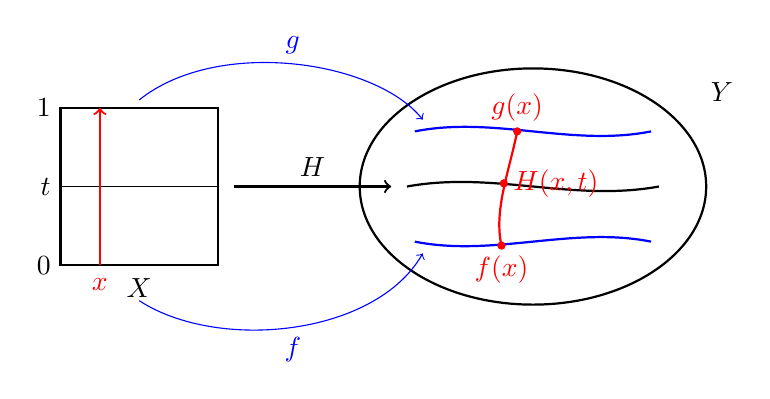
\begin{tikzpicture}[scale=1]
\draw[thick] (0,0) rectangle (2,2);
\node[left] at (0,0) {$0$};
\node[left] at (0,2) {$1$};
\node[left] at (0,1) {$t$};
\draw (0,1) -- (2,1);
\node[below] at (1,-0.05) {$X$};
\draw[red, thick, ->] (0.5,0) -- (0.5,2);
\node[red, below] at (0.5,-0.05) {$x$};
\draw[thick] (6,1) ellipse (2.2 and 1.5);
\node at (8.4,2.2) {$Y$};
\draw[blue, thick] (4.5,0.3) .. controls (5.5,0.1) and (6.5,0.5) .. (7.5,0.3);
\draw[thick] (4.4,1.0) .. controls (5.5,1.2) and (6.5,0.8) .. (7.6,1.0);
\draw[blue, thick] (4.5,1.7) .. controls (5.5,1.9) and (6.5,1.5) .. (7.5,1.7);
\draw[red, thick] (5.6,0.25) .. controls (5.5,0.7) and (5.7,1.2) .. (5.8,1.7);
\fill[red] (5.6,0.25) circle (1.5pt) node[below] {$f(x)$};
\fill[red] (5.63,1.04) circle (1.5pt) node[right] {$H(x,t)$};
\fill[red] (5.8,1.7) circle (1.5pt) node[above] {$g(x)$};
\draw[thick, ->] (2.2,1) -- node[above] {$H$} (4.2,1);
\draw[blue, ->] (1,2.1) .. controls (2,2.9) and (4,2.6) .. (4.6,1.85) node[pos=0.5, above] {$g$};
\draw[blue, ->] (1,-0.45) .. controls (2,-1.1) and (4,-0.9) .. (4.6,0.15) node[pos=0.5, below] {$f$};
\end{tikzpicture}
